% !TEX root = ../presentation.tex
% !BIB program = biber
% !TEX program = xelatex

\section{discussion}

% - It could be interesting to discuss the remaining challenges in integrating the thesis’ range of topics into multi-stage systems for medical domains. This reflects a recurring pattern of clear intra-chapter content, and it would be interesting to discuss further the integration across thesis parts.


% Chapter 4:
% - a point for elaboration of this work would for it to be more prescriptive about how to choose the value of k in the ratio statistic, as it seems to be quite a crucial hyperparameter for practical implementation.

% Chapter 6:
% - Schematically, Figures 6.1 and 6.2 seem inconsistent and could support the text more through a consistent use of colours and labels between them.
% - The chapter doesn’t answer the pressing questions from Chapter 10: What about self-supervised methods for downstream tasks, and should one abandon ship and only focus on self-supervised methods? – this would be interesting to discuss.


\begin{frame}
    \frametitle{The broad picture: The thesis topic since 2020}
    \begin{itemize}
        \item <1-> [2020] \textbf{Project start}
        \begin{itemize} 
            \item <1-> Out-of-distribution detection with generative models: Mysterious new topic.
            \item <1-> Speech representation/recognition: Inflection point between supervised methods and new self-supervised approaches.
        \end{itemize}
        \item <2-> [2024] \textbf{Project end}
        \begin{itemize}
            \item <2-> Out-of-distribution detection is a mature field with a wide range of methods.
            \item <2-> Self-supervised learning is the dominant paradigm in speech recognition - challenged by weak labelling.
            \item <3-> Clinical research is increasingly becoming interested in the use of machine learning.
        \end{itemize}
    \end{itemize}
\end{frame}


\begin{frame}
    \frametitle{What lies ahead}
    
    \begin{itemize}
        \item \highlight{Selective out-of-distribution detection}

        Two pairs of distributions may have identical divergence, but in different dimensions. How do we control features in black-box models?

        \item \highlight{Self-supervised learning in the wild}

        Does the recent progress on academic datasets translate to this real-world setting?

        Speech recognition has been the cornerstone benchmarking task. How do we target spoken language understanding directly?

        \item \highlight{Large language models in medical dialogue}
        
        LLMs will likely play a central role in the future of medical documentation and communication. How do we get a grip of their uncertainty?
    \end{itemize}

    \note[item]{We saw how certain features can dominate an uncertainty score. How do we properly control which features we want to use to detect out-of-distribution data?}
    \note[item]{Self-supervised learning has made great strides in academic benchmarks. How does this translate to real-world settings?}
    \note[item]{LLMs will be important for medical documentation and communication going forward. What does uncertainty look like in this context?}
\end{frame}


\begin{frame}
    \frametitle{The role of uncertainty in an operational decision support system}
    \begin{columns}
        \begin{column}{0.6\textwidth}
            \begin{itemize}
                \item Are true uncertainty estimates really feasible? Pragmatism versus idealism.
                \item Role of explainability compared to uncertainty estimates.
                \item European Parliamentary Research Services \cite{europeanparliament_artificial_2022}:
            \end{itemize}
            \vspace{0.5em}
            \begin{center}
                {\itshape "Future AI solutions for healthcare should be implemented by integrating uncertainty estimation, a relatively new field of research that aims to provide clinicians with clinically useful indications on the degree of confidence in AI predictions"}
            \end{center}
        \end{column}
        \begin{column}{0.4\textwidth}
            \vspace{-2em}
            \begin{figure}[t]
                \centering
                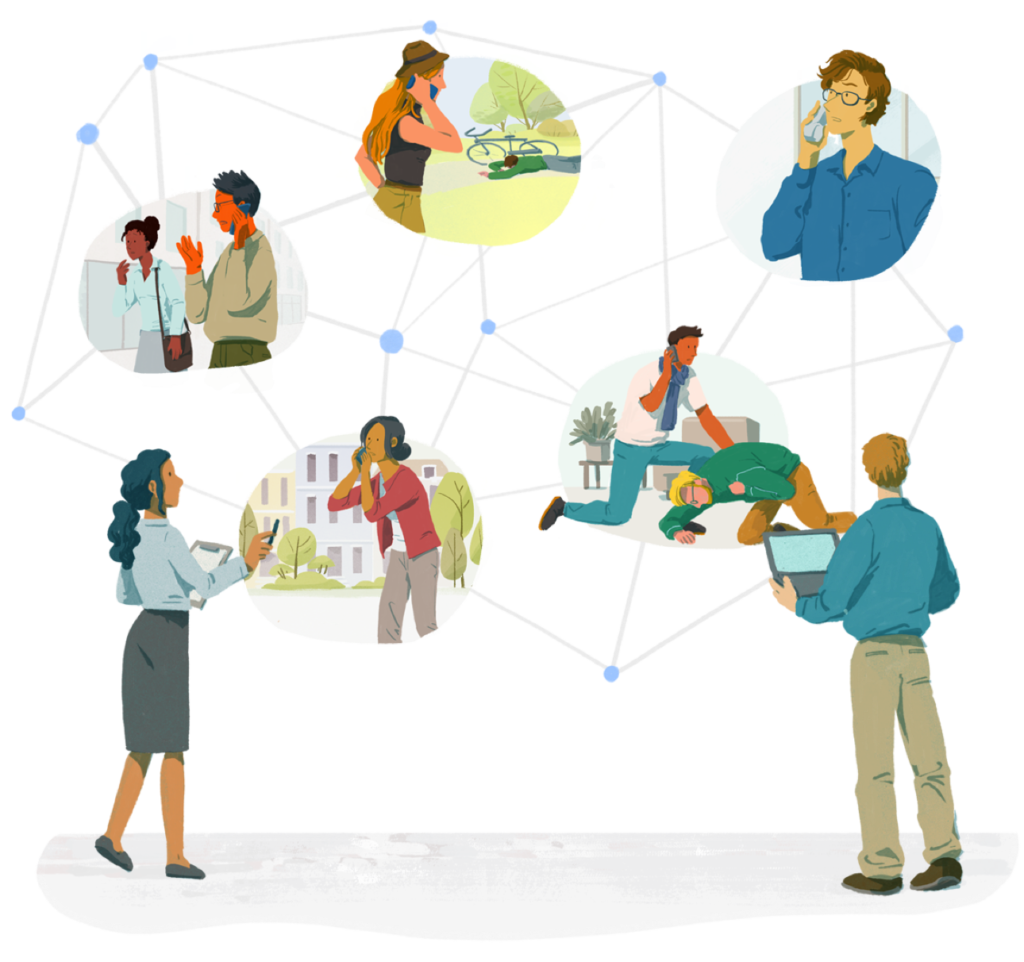
\includegraphics[width=0.9\textwidth]{figures/corti_sketch_conversations.png}
            \end{figure}
        \end{column}
    \end{columns}

    \note[item]{LVMs were difficult to scale to the problems we care about.}
    \note[item]{LVMs did not convincingly outperform more pragmatic approaches (e.g. deferring).}
    % \note[item]{Will uncertainty estimates always be feasible?}
    \note[item]{Bayesian methods, deferring to predict, discriminative uncertainty.}
    \note[item]{What will happen if uncertainty estimates become a regulatory requirement?}
\end{frame}
